%!TEX root = ./intern_report.tex

\newpage
\subsection{Hillnet: An Experimental Attempt at Utilizing ML for Hill Climbing}

\subsubsection{Preprocessing IMU and Velocity Data}

\subsubsection{Data Collection}

% Image: Data Collect
\begin{figure}[H]
    \centering
    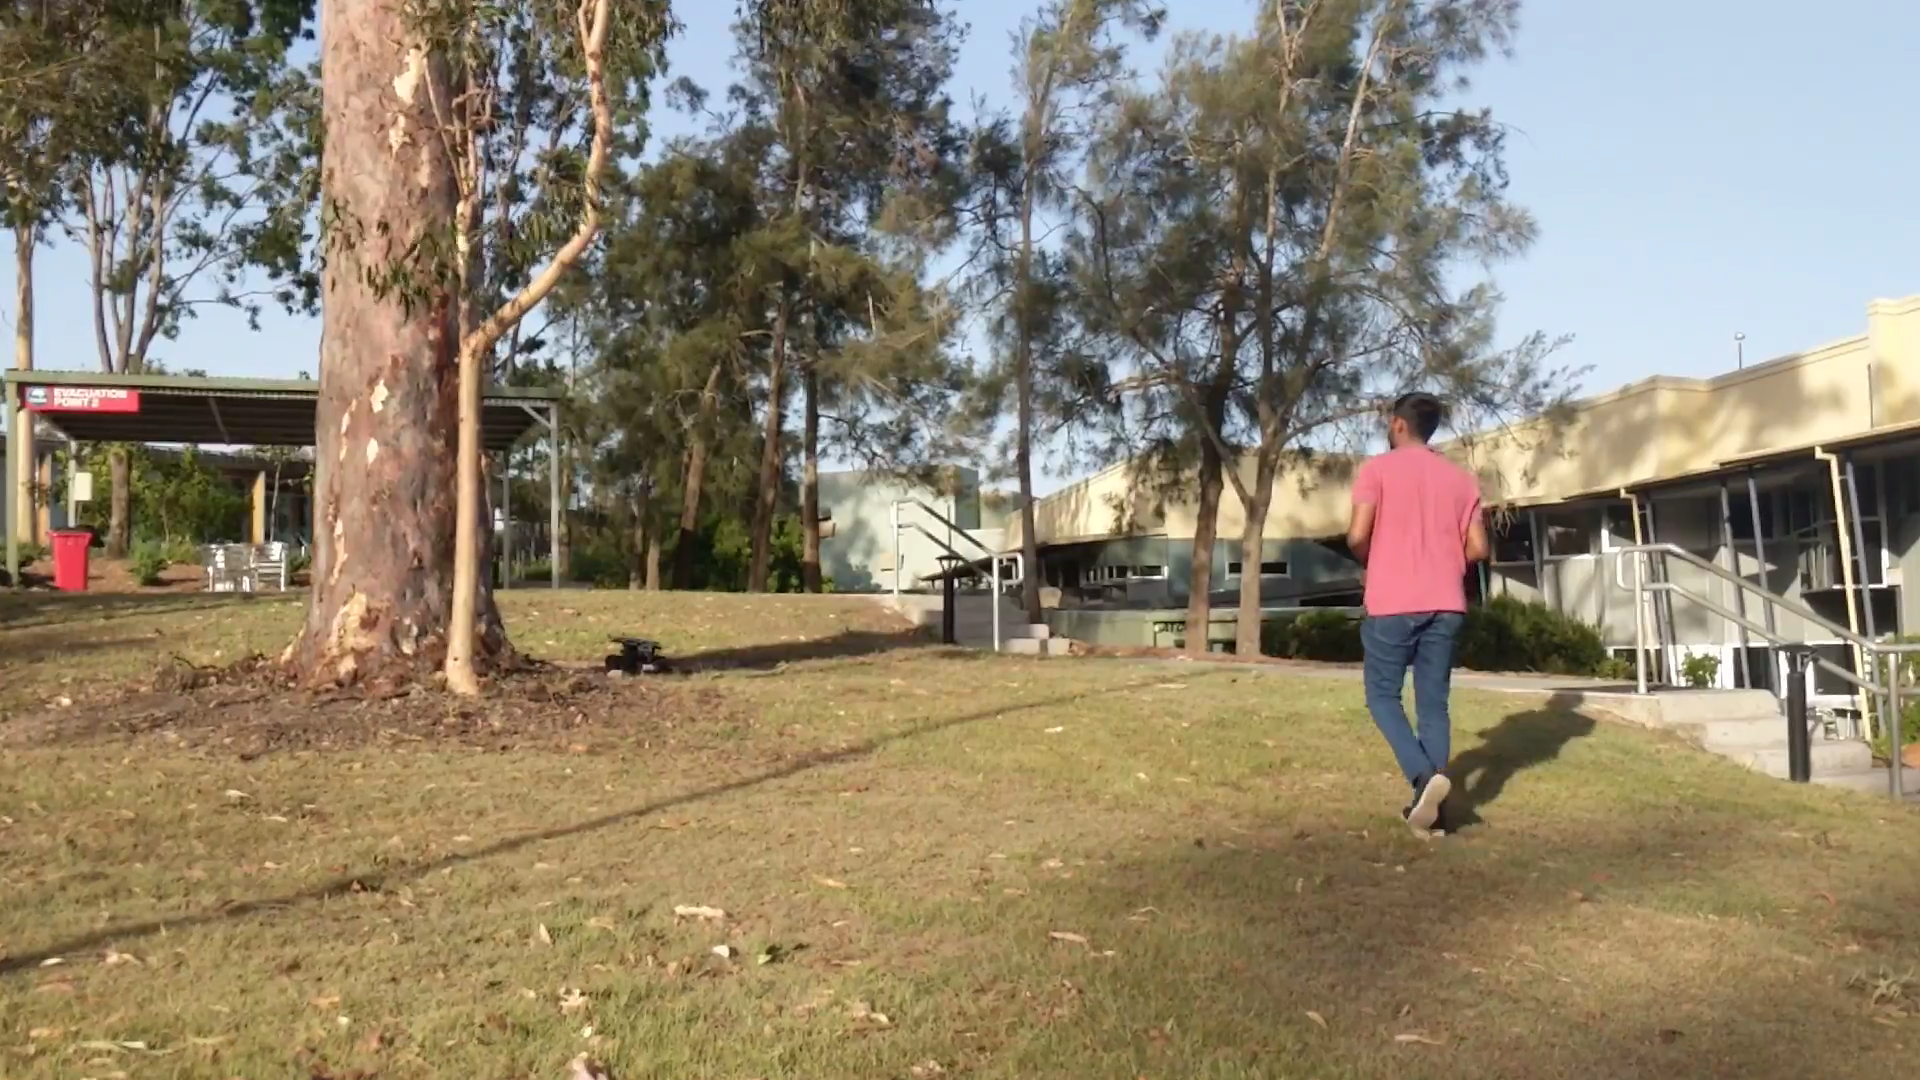
\includegraphics
        [width=8cm]
        {figures/hillnet_data_collect.png}
    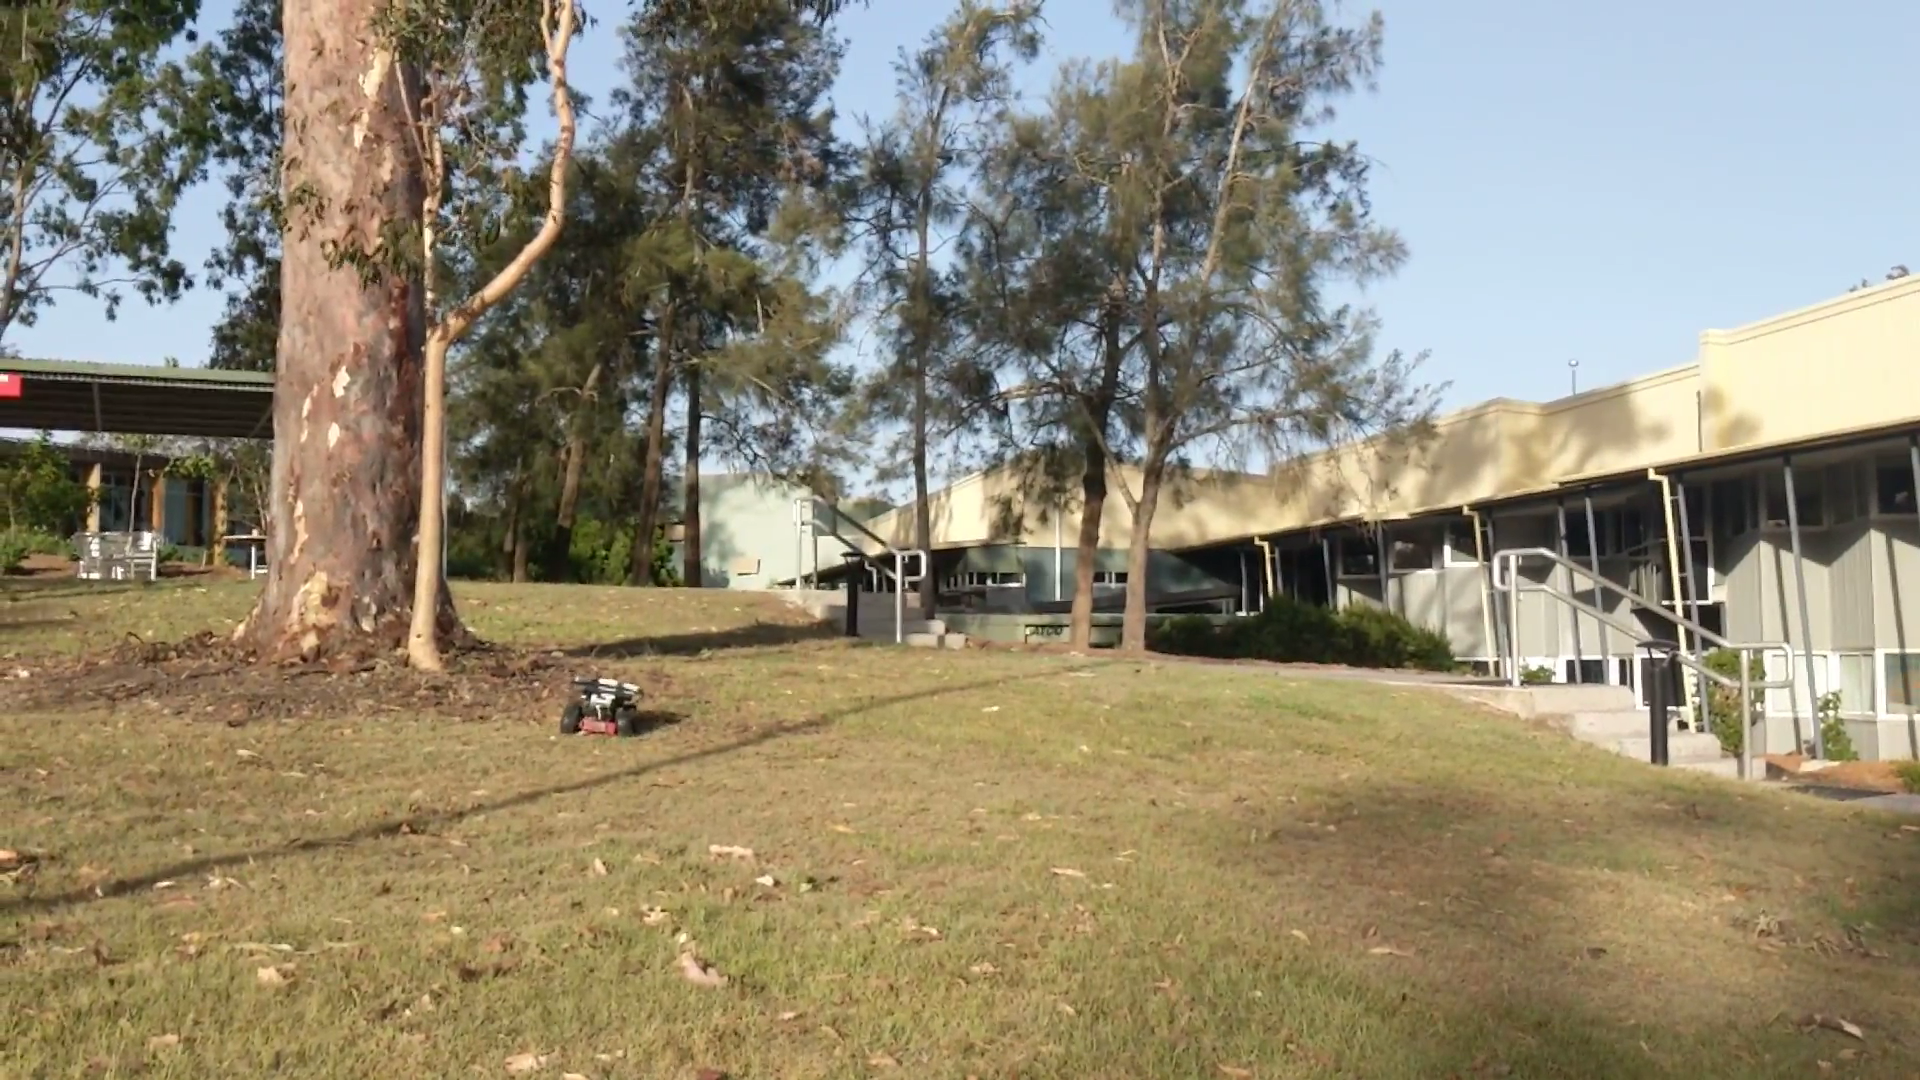
\includegraphics
        [width=8cm]
        {figures/hillnet_data_collect_2.png}
    \caption{Data collection to train hillnet}\vspace{-4mm}
\end{figure}

\subsubsection{Classification Approach}

% Image: Classify Architecture
\begin{figure}[H]
    \centering
    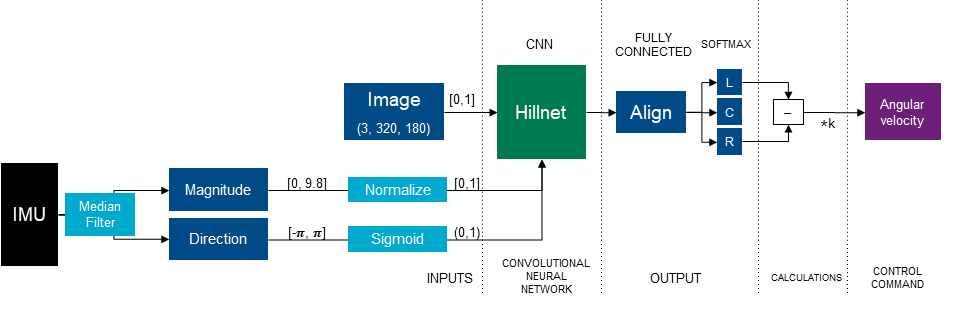
\includegraphics
        [width=16cm]
        {figures/hillnet_classify.PNG}
    \caption{Hillnet Classification Architecture}\vspace{-4mm}
    
\end{figure}

\subsubsection{Regression Approach}

% Image: Regress Architecture
\begin{figure}[H]
    \centering
    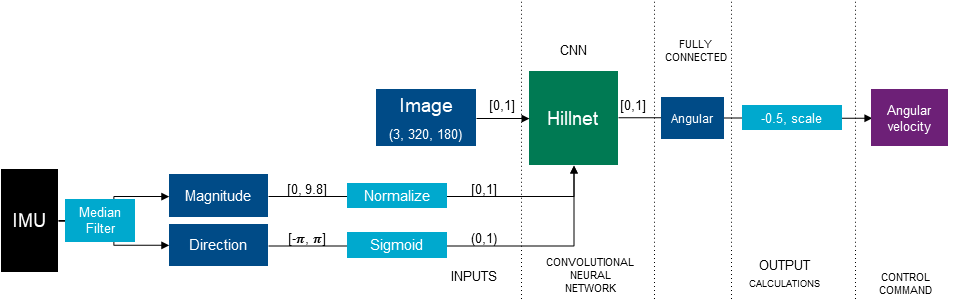
\includegraphics
        [width=16cm]
        {figures/hillnet_regress.PNG}
    \caption{Hillnet Regression Architecture}\vspace{-4mm}
    
\end{figure}

\subsubsection{Merging Scaler and Image Inputs}

% Image: Merge Inputs
\begin{figure}[H]
    \centering
    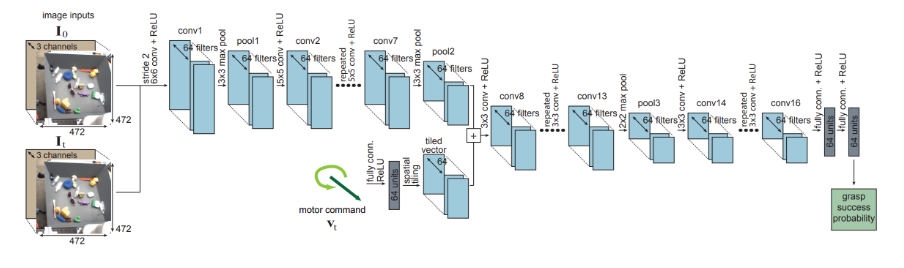
\includegraphics
        [width=16cm]
        {figures/merge_inputs.PNG}
    \caption{Merging by Broadcast and Add}\vspace{-4mm}
    
\end{figure}

\subsubsection{Problems Faced and Solutions}